\section{Introducing the actors: Points and vectors}

\newcommand{\defvF}[2]{\vF \pmat{#1} = \bmat{#2}}
\newcommand{\bvec}[1]{\vec{\mathbf #1}}
\newcommand{\vF}{\vec F}

\bx{ % 1.1.1
    Compute the following vectors by coordinates and sketch what you did:
    \eah{
        \item $\bmat{1\\3} + \bmat{2\\1}$
        \item $2 \bmat{2\\4}$
        \item $\bmat{1\\3} - \bmat{2\\1}$
        \item $\bmat{3\\2} + \bvec e_1$
    }
    \sol{
    \eag{2}{
    \task\
    \begin{minipage}{0.30\linewidth}
        \centering
        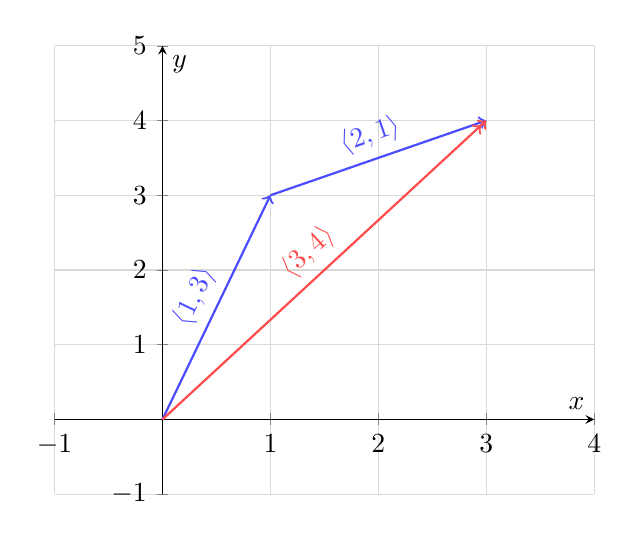
\begin{tikzpicture}
            \begin{axis}[
                axis lines = center,
                xlabel = {$x$},
                ylabel = {$y$},
                xmin = -1, xmax = 4,
                ymin = -1, ymax = 5,
                grid = both,
                major grid style={gray!30},
                minor grid style={gray!10},
                minor tick num = 0,
                ytick distance = 1,
            ]

            \draw[->, thick, blue!70] (axis cs:0,0) -- node[midway, above, sloped] {$\langle 1, 3\rangle$}(axis cs:1,3);
            \draw[->, thick, blue!70] (axis cs:1,3) -- node[midway, above, sloped] {$\langle 2, 1\rangle$}(axis cs:3,4);
            \draw[->>, thick, red!70] (axis cs:0,0) -- node[midway, above, sloped] {$\langle 3, 4\rangle$}(axis cs:3,4);
            \end{axis}
        \end{tikzpicture}
    \end{minipage}

    \task\
    \begin{minipage}{\linewidth}
        \centering
        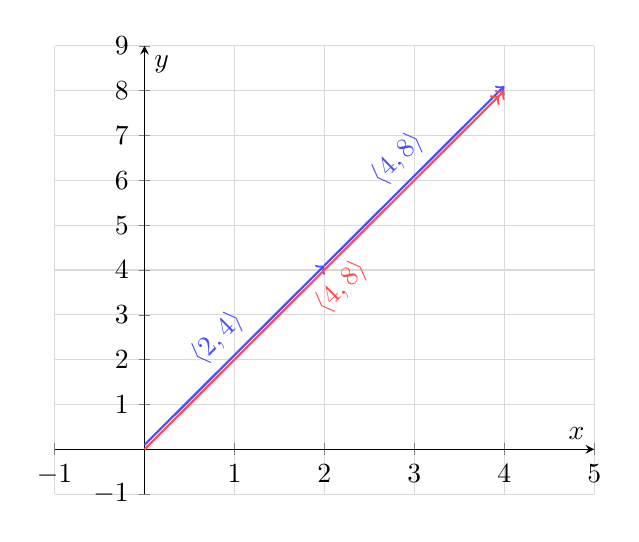
\begin{tikzpicture}
            \begin{axis}[
                axis lines = center,
                xlabel = {$x$},
                ylabel = {$y$},
                xmin = -1, xmax = 5,
                ymin = -1, ymax = 9,
                grid = both,
                major grid style={gray!30},
                minor grid style={gray!10},
                minor tick num = 0,
                ytick distance = 1,
            ]

            \draw[->, thick, blue!70] (axis cs:0,0.1) -- node[midway, above, sloped] {$\langle 2, 4\rangle$}(axis cs:2,4.1);
            \draw[->, thick, blue!70] (axis cs:2,4.1) -- node[midway, above, sloped] {$\langle 4, 8\rangle$}(axis cs:4,8.1);
            \draw[->>, thick, red!70] (axis cs:0,0) -- node[midway, below, sloped] {$\langle 4, 8\rangle$}(axis cs:4,8);
            \end{axis}
        \end{tikzpicture}
    \end{minipage}

    \task\
     \begin{minipage}{\linewidth}
        \centering
        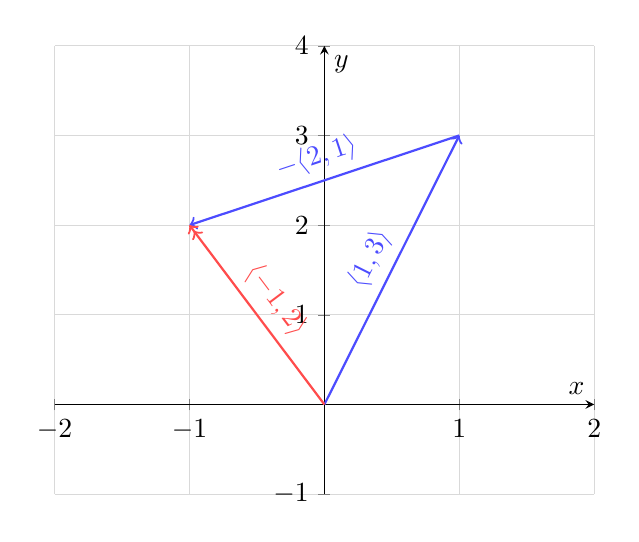
\begin{tikzpicture}
            \begin{axis}[
                axis lines = center,
                xlabel = {$x$},
                ylabel = {$y$},
                xmin = -2, xmax = 2,
                ymin = -1, ymax = 4,
                grid = both,
                major grid style={gray!30},
                minor grid style={gray!10},
                minor tick num = 0,
                ytick distance = 1,
            ]

            \draw[->, thick, blue!70] (axis cs:0,0) -- node[midway, above, sloped] {$\langle 1, 3\rangle$}(axis cs:1,3);
            \draw[->, thick, blue!70] (axis cs:1,3) -- node[midway, above, sloped] {$-\langle 2, 1\rangle$}(axis cs:-1,2);
            \draw[->>, thick, red!70] (axis cs:0,0) -- node[midway, above, sloped] {$\langle -1, 2\rangle$}(axis cs:-1,2);
            \end{axis}
        \end{tikzpicture}
    \end{minipage}

    \task\
     \begin{minipage}{\linewidth}
        \centering
        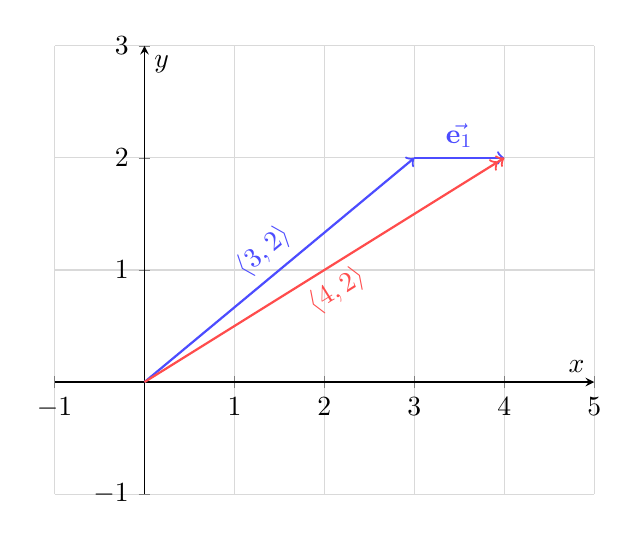
\begin{tikzpicture}
            \begin{axis}[
                axis lines = center,
                xlabel = {$x$},
                ylabel = {$y$},
                xmin = -1, xmax = 5,
                ymin = -1, ymax = 3,
                grid = both,
                major grid style={gray!30},
                minor grid style={gray!10},
                minor tick num = 0,
                ytick distance = 1,
            ]

            \draw[->, thick, blue!70] (axis cs:0,0) -- node[midway, above, sloped] {$\langle 3, 2\rangle$}(axis cs:3 ,2);
            \draw[->, thick, blue!70] (axis cs:3,2) -- node[midway, above, sloped] {$\vec{\mathbf e_1}$}(axis cs:4,2);
            \draw[->>, thick, red!70] (axis cs:0,0) -- node[midway, below, sloped] {$\langle 4, 2\rangle$}(axis cs:4,2);
            \end{axis}
        \end{tikzpicture}
    \end{minipage}
    }}
}

\bx{ % 1.1.2
    Compute the following vectors:
    \eah{
        \item $\bmat{3 \\ \pi \\ 1} + \bmat{1 \\ -1 \\ \sqrt2}$
        \item $\bmat{1 \\ 4 \\ c \\ 2} + \bvec e_2$
        \item $\bmat{1 \\ 4 \\ c \\ 2} - \bvec e_4$
    }
}

\bx{ % 1.1.3
    In the following, translate the word “in” by the appropriate symbol: $\in$ (element of) or $\subset$ (subset of). 
    \eag{2}{
        \task A vector $\bvec v$ in $\R^3$
        \task A line $L$ in $\R^2$
        \task A curve $C$ in $\R^3$
        \task A point $\mathbf x$ in $\C^2$
        \task A sequence of nested balls $B_0$ in $B_1$ in $B_2 \ cdots$
    }
}  

\bx{ % 1.1.4
    \ea{
        \item Name the two trivial subspaces of $\R^n$.
        \item Let $S^1 \subset \R^2$ be the unit circle, of equation $x^2 + y^2 = 1$. Do there exist any elements of $S^1$ whose sum is an element of the set?
    }
}

\bx{ % 1.1.5
    Using the sum notation (discussed in Section 0.1), write the following vectors as the sum of multiple standard basis vectors.
    \eah{
        \item $\bmat{1 \\ 1 \\ \vdots \\ 1 \\ 1}$,
        \item $\bmat{1 \\ 2 \\ \vdots \\ n-1 \\ n}$,
        \item $\bmat{0 \\ 0 \\ 3 \\ 4 \\ \vdots \\ n-1 \\ n}$
    }
}

\bx{ % 1.1.6
    Sketch the following vector fields:
    \eag{3}{
    \task $\defvF{x \\ y}{0 \\ 1}$
    \task $\defvF{x \\ y}{x \\ 0}$
    \task $\defvF{x \\ y}{x \\ y}$
    \task $\defvF{x \\ y}{x \\ -y}$
    \task $\defvF{x \\ y}{y \\ x}$
    \task $\defvF{x \\ y}{-y \\ x}$
    \task $\defvF{x \\ y}{y \\ x-y}$
    \task $\defvF{x \\ y}{x-y \\ x+y}$
    \task $\defvF{x \\ y}{x^2-y-1 \\ x-y}$
    }
}

\bx{ % 1.1.7
    Sketch the following vector fields:
    \eag{3}{
    \task $\defvF{x \\ y \\ z}{0 \\ 0 \\ x^2+y^2}$
    \task $\defvF{x \\ y \\ z}{y \\ -x \\ -z}$
    \task $\defvF{x \\ y \\ z}{x-y \\ x+y \\ -z}$
    }
}

\bx{ % 1.1.8
    Suppose that water is flowing through a pipe of radius $r$, with speed $r^2 -a^2$, where $a$ is the distance to the axis of the pipe.
    \ea{
        \item Write a vector field describing the flow if the pipe is the direction of the $z$-axis.
        \item Write the vector field describing the flow if the axis of the pipe is the unit circle in the $(x, y)$-plane
    }
}

\bx{ % 1.1.9
    Show that the set of complex numbers $\{z|\mathrm{Re}(wz) = 0\}$ with fixed $w\in\C$ is a subspace of $\R^2 = \C$. Describe this subspace.
}
